% ============================================================
% Rapport Technique --- Rapport 7
% QLoRA Fine-Tuning of Gemma-2-2B-IT for IaC Security
% Remediation: Methodology, Execution, and Integration Path
%
% Ahmedou Yahye Kheyri
% Supervised by: Hala Bezine
% Faculté des Sciences de Sfax --- Master MRSI
% 2025--2026
% ============================================================

\documentclass[12pt, a4paper]{report}

% ---- Encoding & Language ----
\usepackage[utf8]{inputenc}
\usepackage[T1]{fontenc}
\usepackage[english]{babel}

% ---- Layout ----
\usepackage[
  top=2.5cm, bottom=2.5cm,
  left=3cm,  right=2.5cm
]{geometry}
\usepackage{setspace}
\onehalfspacing
\setlength{\parindent}{1.2em}
\setlength{\parskip}{0.4em}
\setlength{\headheight}{14pt}

% ---- Fonts ----
\usepackage{lmodern}
\usepackage{microtype}

% ---- Math ----
\usepackage{amsmath}
\usepackage{amssymb}

% ---- Graphics & Tables ----
\usepackage{graphicx}
\usepackage{float}
\usepackage{booktabs}
\usepackage{tabularx}
\usepackage{multirow}
\usepackage{longtable}
\usepackage{array}
\usepackage[table,xcdraw]{xcolor}

% ---- Code Listings ----
\usepackage{listings}
\usepackage{lstautogobble}

\definecolor{codegreen}{rgb}{0.0,0.5,0.0}
\definecolor{codegray}{rgb}{0.5,0.5,0.5}
\definecolor{codepurple}{rgb}{0.58,0,0.82}
\definecolor{backcolour}{rgb}{0.97,0.97,0.97}
\definecolor{codeblue}{rgb}{0.0,0.0,0.7}

\lstdefinestyle{iacstyle}{
  backgroundcolor=\color{backcolour},
  commentstyle=\color{codegreen}\itshape,
  keywordstyle=\color{codeblue}\bfseries,
  stringstyle=\color{codepurple},
  basicstyle=\ttfamily\small,
  breakatwhitespace=false,
  breaklines=true,
  captionpos=b,
  keepspaces=true,
  numbers=left,
  numbersep=6pt,
  numberstyle=\tiny\color{codegray},
  showspaces=false,
  showstringspaces=false,
  showtabs=false,
  tabsize=2,
  frame=single,
  rulecolor=\color{gray!40},
  autogobble=true
}
\lstset{style=iacstyle}

\lstdefinestyle{celloutput}{
  backgroundcolor=\color{gray!5},
  basicstyle=\ttfamily\footnotesize,
  breaklines=true,
  breakatwhitespace=false,
  captionpos=b,
  keepspaces=true,
  showspaces=false,
  showstringspaces=false,
  frame=single,
  rulecolor=\color{gray!40},
  autogobble=false
}

% ---- TikZ ----
\usepackage{tikz}
\usetikzlibrary{shapes.geometric, arrows.meta, positioning, fit, backgrounds, calc}

% ---- Colors (academic, sober) ----
\definecolor{titleblue}{RGB}{40, 70, 130}
\definecolor{softgray}{RGB}{240, 240, 240}

% ---- Headers & Footers ----
\usepackage{fancyhdr}
\pagestyle{fancy}
\fancyhf{}
\fancyhead[L]{\small\leftmark}
\fancyhead[R]{\small\thepage}
\fancyfoot[C]{\small Ahmedou Yahye Kheyri --- Faculté des Sciences de Sfax}
\renewcommand{\headrulewidth}{0.4pt}
\renewcommand{\footrulewidth}{0.2pt}

% ---- Hyperlinks ----
\usepackage[
  colorlinks=true,
  linkcolor=titleblue,
  citecolor=titleblue,
  urlcolor=titleblue,
  bookmarks=true,
  bookmarksnumbered=true
]{hyperref}
\usepackage{url}

% ---- Caption ----
\usepackage[font=small,labelfont=bf]{caption}
\usepackage{subcaption}

% ---- Boxes ----
\usepackage{tcolorbox}
\tcbuselibrary{breakable, skins}

\newtcolorbox{infobox}[1][]{
  colback=gray!5!white, colframe=gray!60!black,
  fonttitle=\bfseries, title={#1},
  breakable, enhanced
}

\newtcolorbox{cellbox}[1][]{
  colback=blue!3!white, colframe=titleblue,
  fonttitle=\bfseries\small, title={#1},
  breakable, enhanced, arc=2pt
}

% ---- Chapter style ----
\usepackage{titlesec}
\titleformat{\chapter}[display]
  {\normalfont\huge\bfseries\color{titleblue}}
  {\chaptertitlename\ \thechapter}{16pt}{\Huge}
\titlespacing*{\chapter}{0pt}{-10pt}{20pt}

% ---- Acronyms ----
\usepackage[acronym,toc]{glossaries}
\makeglossaries
\newacronym{iac}{IaC}{Infrastructure as Code}
\newacronym{llm}{LLM}{Large Language Model}
\newacronym{lora}{LoRA}{Low-Rank Adaptation}
\newacronym{qlora}{QLoRA}{Quantized Low-Rank Adaptation}
\newacronym{peft}{PEFT}{Parameter-Efficient Fine-Tuning}
\newacronym{sft}{SFT}{Supervised Fine-Tuning}
\newacronym{cwe}{CWE}{Common Weakness Enumeration}
\newacronym{rag}{RAG}{Retrieval-Augmented Generation}
\newacronym{gguf}{GGUF}{GPT-Generated Unified Format}
\newacronym{api}{API}{Application Programming Interface}
\newacronym{hf}{HF}{Hugging Face}
\newacronym{vram}{VRAM}{Video Random-Access Memory}
\newacronym{nf4}{NF4}{4-bit NormalFloat}

% ============================================================
\begin{document}
% ============================================================

% ---- Title Page ----
\begin{titlepage}
  \centering

  \vspace*{2.5cm}
  {\small Ministère de l'Enseignement Supérieur, de la Recherche Scientifique
   et de la Technologie}\\[4pt]
  {\small Université de Sfax \enspace\textbar\enspace Faculté des Sciences de Sfax}\\[4pt]
  {\small Département d'Informatique \enspace\textbar\enspace Master MRSI}

  \vspace{2.5cm}

  \noindent\rule{\linewidth}{0.6pt}\\[0.8cm]

  {\Large\bfseries\color{titleblue}
    QLoRA Fine-Tuning of Gemma-2-2B-IT for\\[6pt]
    Infrastructure as Code Security Remediation
  }\\[0.4cm]

  {\normalsize\itshape Methodology, Kaggle Execution, and Integration Path}\\[0.6cm]

  \noindent\rule{\linewidth}{0.6pt}

  \vspace{0.6cm}
  {\normalsize\itshape Technical Report --- Rapport 7}

  \vspace{3cm}
  \begin{minipage}[t]{0.45\textwidth}
    \raggedright
    {\small\bfseries Prepared by}\\[4pt]
    {\normalsize Ahmedou Yahye Kheyri}\\[2pt]
  \end{minipage}
  \hfill
  \begin{minipage}[t]{0.45\textwidth}
    \raggedleft
    {\small\bfseries Supervised by}\\[4pt]
    {\normalsize Pr.\ Hala Bezine}\\[2pt]
  \end{minipage}

  \vfill
  {\small\textit{Keywords:}\enspace
   Fine-Tuning \textbullet\
   QLoRA \textbullet\
   Gemma-2 \textbullet\
   Infrastructure as Code \textbullet\
   Security Smells \textbullet\
   Kaggle}\\[1.2cm]

  {\small Academic Year 2025--2026}
  \vspace{1cm}

\end{titlepage}

% ---- Abstract ----
\chapter*{Abstract}
\addcontentsline{toc}{chapter}{Abstract}

This technical report documents a \emph{first, preliminary} fine-tuning
experiment conducted within the broader agentic \gls{iac} security framework
introduced in \emph{Rapport 2}. The experiment is deliberately small in scope:
a single run, a small open-weight model (\(\approx\)~2~B parameters), a
4{,}050-record subset of our scraped data, one epoch, and no hyperparameter
search. Its purpose is not to deliver a state-of-the-art model but to
validate that the training pipeline works end to end and to surface the
issues that must be addressed before any scaled experiment is attempted.

We describe (i) the composition of the training data --- a 31{,}748-record
scanner-validated dataset obtained through our custom \gls{iac} security
scraper; (ii) the data preparation pipeline that extracts a 4{,}050-record
\emph{gold subset} used in this first run (roughly 38~\% of the available
scanner-validated records, sharply filtered for length and non-noop changes);
(iii) the \gls{qlora} training methodology applied to
\texttt{google/gemma-2-2b-it} on Kaggle's T4~x2 tier (one of the two
available T4 GPUs used by our single-process script), where we observed
a training loss of 0.528 and an evaluation loss of 0.467 in 1~h~47~min for one
epoch; (iv) a qualitative inspection of the resulting adapter on only three
held-out test samples; and (v) the integration path that remains to be
executed --- adapter merging, \gls{gguf} conversion, and local Ollama
serving.

The report is a standalone technical document but remains tightly coupled to
the global thesis project: once merged and served locally, the fine-tuned
adapter is intended to serve as the candidate \gls{llm} for the \emph{Config
B} evaluation condition of the experimental plan. At the time of writing,
that evaluation has not yet been carried out; only Config A (Checkov alone)
has measured results. All Kaggle notebook cells, training hyperparameters,
and output logs are reproduced verbatim so that the experiment can be
replayed or extended.

\bigskip
\noindent\textbf{Keywords:} Fine-Tuning, QLoRA, Gemma-2, Infrastructure as Code,
Security Smells, Kaggle, Parameter-Efficient Fine-Tuning.

% ---- TOC ----
\tableofcontents
\listoffigures
\listoftables

\printglossary[type=\acronymtype, title=List of Acronyms]

% ============================================================
\chapter{Introduction and Positioning}
% ============================================================

\section{Context in the Overall Project}

The master's thesis project introduces an \emph{agentic framework} for
\gls{iac} security analysis and remediation. Seven modules cooperate under
a central orchestrator: a contextual analyzer, a knowledge base, a
\gls{rag} retriever, a fix generator, an external validator (Checkov,
GLITCH, Terrascan), a patch formatter, and the orchestrator itself. A
detailed architecture and evaluation methodology are given in
\emph{Rapport 2}; early experimental results (Config A baseline, Checkov
alone) are reported in its Chapter~6.

Among those modules, the \textbf{fix generator} is the only component whose
quality is bounded by the underlying \gls{llm} rather than by deterministic
software. In the baseline configuration, the framework can call any
OpenAI-, Anthropic-, or Ollama-compatible backend. For local deployment and
reproducibility we rely on Ollama serving small open-weight models such as
Gemma-3-4B and Gemma-4-e2B. Informal tests on this baseline suggested two
points of concern that motivate the present experiment:

\begin{itemize}
  \item \textbf{Generic behaviour}: the off-the-shelf \gls{llm} produces
  plausible fixes but, in our limited manual checks, did not always target
  the specific \gls{cwe} category reported by the analyzer. A systematic
  measurement remains to be done.
  \item \textbf{Latency}: on a single laptop CPU we observed roughly 320
  seconds per fix with the Gemma-4-e2B model, which would make a full
  dataset evaluation with self-consistency sampling impractical on the
  current hardware.
\end{itemize}

A plausible direction is to fine-tune a small open-weight model on the
data we already scraped. This report documents a \emph{first, exploratory}
attempt in that direction, carried out on Kaggle's free GPU tier.

\section{Why Fine-Tuning, Why a Small Model}

Fine-tuning adapts a pretrained model to a narrow downstream distribution.
Compared to in-context prompting alone, supervised fine-tuning on curated
(insecure, fixed) pairs is \emph{expected} to offer two advantages: the
model may learn domain vocabulary that is sparse in general pretraining
corpora (scanner rule identifiers, provider-specific HCL patterns,
Kubernetes security-context fields), and the instruction-following
behaviour may become more consistent in output format (a compilable
\gls{iac} block rather than a discursive explanation). Whether these
advantages actually materialise for our setup is an empirical question
that this first run cannot yet answer.

A small model (\(\leq\) 3~B parameters) is chosen deliberately for this
first experiment. The agentic framework targets \emph{local} inference as
part of security audits that cannot route code through a third-party
\gls{api}. Gemma-2-2B-IT is small enough to fit on an NVIDIA T4 (16~GB)
with 4-bit quantisation, can in principle be merged into a standalone
\gls{gguf} file of roughly 1.5~GB, and is expected to run at usable
latency inside Ollama on a commodity laptop. A 2~B model is modest by
current standards and is chosen for tractability rather than for expected
peak quality; larger candidates (Qwen2.5-Coder-3B, Gemma-2-9B) are
deferred to a subsequent iteration.

\section{Contributions of This Report}

The contributions of this report are modest and should be read as a
first iteration:

\begin{enumerate}
  \item A reproducible three-script training pipeline
        (\texttt{01\_prepare\_dataset.py}, \texttt{02\_train\_qlora.py},
         \texttt{03\_inference.py}) under
         \texttt{Code/training/trainning/}.
  \item One \gls{qlora} fine-tuning run on
        \texttt{google/gemma-2-2b-it}, executed on Kaggle's free
        T4~x2 tier under the constraints imposed by that environment
        (single-process script using one of the two T4 devices,
        9-hour session limit, gated model access).
  \item The observed training metrics from that single run (loss curves,
        runtime, adapter size) and a qualitative look at only three
        held-out test samples, with a candid discussion of the label
        noise we encountered.
  \item A proposed integration path --- not yet executed --- that would
        turn the trained \gls{lora} adapter into a deployable Ollama
        model usable by the framework's existing \texttt{FixGenerator}
        class without source-code changes.
\end{enumerate}

Nothing in this report should be read as a quantitative comparison
against baselines, and the model produced here has not yet been
evaluated inside the full agentic pipeline.

\section{Structure of the Report}

Chapter~\ref{ch:background} provides the necessary background on \gls{lora}
and \gls{qlora}. Chapter~\ref{ch:dataset} describes the dataset used for
training, its origin, statistics, and filtering pipeline.
Chapter~\ref{ch:methodology} presents the fine-tuning methodology
(model choice, hyperparameters, prompt format).
Chapter~\ref{ch:execution} reproduces the Kaggle execution in full,
cell by cell, with captured output.
Chapter~\ref{ch:results} analyses training metrics and the qualitative
inference test.
Chapter~\ref{ch:discussion} discusses limitations, particularly dataset
label noise, and Chapter~\ref{ch:next} outlines the remaining integration
steps required to plug the fine-tuned model into the full agentic pipeline.

% ============================================================
\chapter{Background}
\label{ch:background}
% ============================================================

\section{Low-Rank Adaptation (LoRA)}

\gls{lora}~(Hu~\emph{et al.}, 2021)\footnote{E.~Hu \emph{et al.},
\emph{LoRA: Low-Rank Adaptation of Large Language Models}, arXiv:2106.09685.}
is a parameter-efficient fine-tuning method
that freezes the original weights \(W_0 \in \mathbb{R}^{d \times k}\) of a
pretrained model and learns a low-rank update
\(\Delta W = B A\), with \(B \in \mathbb{R}^{d \times r}\) and
\(A \in \mathbb{R}^{r \times k}\) for a small rank \(r \ll \min(d,k)\).
At inference time the effective weight becomes \(W = W_0 + \Delta W\).

Only \(A\) and \(B\) are updated during training, which reduces the number
of trainable parameters by several orders of magnitude. For Gemma-2-2B
with \(r=16\) applied to all attention projection matrices, the trainable
parameter count is approximately 9.3~million out of 2.6~billion --- a
trainable fraction of 0.35~\%. The resulting adapter file is 25~MB instead
of the 5~GB of the full model.

\section{Quantised LoRA (QLoRA)}

\gls{qlora}~(Dettmers~\emph{et al.}, 2023)\footnote{T.~Dettmers \emph{et al.},
\emph{QLoRA: Efficient Finetuning of Quantized LLMs}, arXiv:2305.14314.}
combines \gls{lora} with 4-bit
quantisation of the \emph{base} weights. Forward passes decompress each
weight tile on demand, keep activations in 16-bit precision for numerical
stability, and route gradients exclusively through the low-rank adapter.
The most common quantisation scheme is \gls{nf4} with double-quantisation
of the scaling constants.

The memory footprint of a 2-billion-parameter model collapses from
\(\approx\)~10~GB (fp32) or 5~GB (fp16) to roughly 1.6~GB with \gls{nf4}.
Combined with gradient checkpointing, this makes it feasible to fine-tune
such a model on a single 16~GB T4, which is precisely the environment
available on Kaggle's free tier.

\section{Supervised Fine-Tuning for Code Repair}

Our task is a form of \gls{sft}~(Ouyang~\emph{et al.}, 2022)\footnote{L.~Ouyang
\emph{et al.}, \emph{Training Language Models to Follow Instructions with
Human Feedback}, NeurIPS 2022.} where the
model receives an instruction prompt and produces a target completion.
The instruction describes the detected security smells; the completion is
the human-written fixed version of the script. The training objective is
the usual causal-language-modelling loss computed only on the completion
tokens when a chat template is applied.

Unlike classical code generation, our setting is closer to
\emph{code-to-code translation}: the model sees broken code and must emit
valid code that preserves functional equivalence while removing the
security smell. This narrow, constrained task is well suited to
parameter-efficient fine-tuning with limited data.

% ============================================================
\chapter{Dataset}
\label{ch:dataset}
% ============================================================

\section{Origin: the Scraping Module}

The training data comes from a custom scraper we developed and documented
in \texttt{Code/scraping/}. The scraper combines five complementary
strategies to collect (insecure, fixed) \gls{iac} pairs from public sources:

\begin{enumerate}
  \item \textbf{GitHub Commit Search} with date-window partitioning to
        bypass the 1{,}000-result hard cap. Each commit whose message
        mentions security-related keywords is inspected; for every
        \gls{iac} file changed in the commit, the version before and
        after the fix is downloaded through the Core API.
  \item \textbf{GHArchive discovery}: hourly dumps of all public GitHub
        events are pre-filtered by repository-name regex before resolving
        push events, which bypasses the Search \gls{api} quota entirely.
  \item \textbf{Scanner test suites}: Checkov, KICS, and tfsec all ship
        with paired ``failed'' and ``passed'' example files. These are a
        natural source of clean before/after pairs.
  \item \textbf{Known vulnerable repositories}: TerraGoat,
        Kubernetes-Goat, and OWASP WrongSecrets contribute
        intentionally insecure files.
  \item \textbf{Scanner-validated labels}: a post-processing pass runs
        Checkov, tfsec, and KICS on every record and attaches
        \texttt{validated\_smells\_before} / \texttt{validated\_smells\_after}
        lists. This produces \emph{scanner-confirmed} ground-truth labels
        suitable for supervised training.
\end{enumerate}

The scraper was run for several days with progress checkpointing,
SHA-256 deduplication, and exponential-backoff retries to cope with
GitHub rate limits. Full implementation details are in
\texttt{Code/scraping/README.md}.

\section{Version 1 Statistics}

The frozen \emph{version~1} dataset
(\texttt{scraping/output/dataset\_v1\_validated.jsonl}, 322~MB) contains
31{,}748 records after global deduplication. Table~\ref{tab:v1-stats}
summarises its composition.

\begin{table}[H]
  \centering
  \caption{Dataset v1 overall statistics.}
  \label{tab:v1-stats}
  \small
  \begin{tabular}{lr}
    \toprule
    \textbf{Property} & \textbf{Value} \\
    \midrule
    Total records (deduplicated) & 31{,}748 \\
    Records with fix (\texttt{has\_fix}=True) & 16{,}362 (51.5~\%) \\
    Scanner-validated records & 10{,}791 (34.0~\%) \\
    Source repositories & $>$~2{,}000 \\
    Security smell types & 18 \\
    Pre-existing train / val / test split & 25{,}383 / 3{,}189 / 3{,}176 \\
    Average combined code length & 5{,}760 characters \\
    Maximum combined code length & 263{,}965 characters \\
    \bottomrule
  \end{tabular}
\end{table}

\begin{table}[H]
  \centering
  \caption{Version~1 breakdown by \gls{iac} tool.}
  \label{tab:v1-by-tool}
  \small
  \begin{tabular}{lrr}
    \toprule
    \textbf{\gls{iac} tool} & \textbf{Records} & \textbf{Share} \\
    \midrule
    Terraform       & 15{,}863 & 50.0~\% \\
    Kubernetes      &  8{,}919 & 28.1~\% \\
    Ansible         &  4{,}161 & 13.1~\% \\
    Docker          &  2{,}333 &  7.3~\% \\
    CloudFormation  &    472   &  1.5~\% \\
    \bottomrule
  \end{tabular}
\end{table}

The smell distribution is heavily skewed toward Docker- and
Kubernetes-centric issues: \texttt{missing\_resource\_limits}~(4{,}505),
\texttt{unpinned\_base\_image}~(3{,}429), \texttt{overly\_permissive\_cidr}
(1{,}614), \texttt{latest\_image\_tag}~(1{,}009), and
\texttt{capabilities\_added}~(884) account for most of the data.
Credential-related smells are under-represented ($<$~500 records each)
because commits that fix hard-coded secrets are often held in private
repositories or heavily redacted.

\section{Filtering Pipeline for Supervised Fine-Tuning}

Raw records are not immediately usable for training. The preparation
script \texttt{01\_prepare\_dataset.py} applies six filters in sequence
(Table~\ref{tab:filter-pipeline}).

\begin{table}[H]
  \centering
  \caption{Filter pipeline from 31{,}748 raw records to the gold training subset.}
  \label{tab:filter-pipeline}
  \small
  \begin{tabular}{lrr}
    \toprule
    \textbf{Filter} & \textbf{Remaining} & \textbf{Kept} \\
    \midrule
    Input (all validated records)         & 31{,}748 & 100.0~\% \\
    \texttt{has\_fix} = \texttt{True}     & 16{,}362 & 51.5~\% \\
    Scanner-validated (\texttt{gold\_only}=True) & $\sim$10{,}791 & 34.0~\% \\
    Non-empty \texttt{code\_before} and \texttt{code\_after} & $\sim$10{,}500 & --- \\
    Combined length $<$~8{,}000 chars     & $\sim$5{,}500 & --- \\
    Non-noop fix (\texttt{before} $\neq$ \texttt{after}) & 4{,}050 & 12.76~\% \\
    Pre-existing train split (80~\%)      & \textbf{3{,}227} & --- \\
    \bottomrule
  \end{tabular}
\end{table}

The combined length cap is a direct consequence of the \gls{vram} budget:
at a maximum sequence length of 2{,}048 tokens, the attention memory grows
as \(O(n^2)\) and longer contexts are unlikely to fit alongside the model
state on a T4. The scanner-validated filter is the most aggressive (it
discards roughly two thirds of fix pairs); it ensures that the
\texttt{code\_before} is flagged as vulnerable by at least one static
analyser, rather than being selected only from keywords in the commit
message. This filter acts only at the \emph{record} level and does not
guarantee that the recorded diff addresses the same vulnerability --- a
limitation we return to in Chapter~\ref{ch:discussion}.

The 4{,}050-record gold subset used in this experiment is, by design, a
small fraction of what is available. The same pipeline can produce a
larger (but noisier) corpus of up to \(\approx\)~10{,}791 scanner-validated
records if the length and non-noop filters are relaxed; exploring that
regime is deferred to a later iteration.

\section{Gold Subset: Training-Ready Statistics}

After filtering, the resulting corpus counts 4{,}050 records
(3{,}227 train, 411 validation, 412 test).
Table~\ref{tab:gold-distribution} shows a much more balanced distribution
by \gls{iac} tool than the raw dataset.

\begin{table}[H]
  \centering
  \caption{Gold subset distribution after filtering.}
  \label{tab:gold-distribution}
  \small
  \begin{tabular}{lrr}
    \toprule
    \textbf{Tool} & \textbf{Records} & \textbf{Share} \\
    \midrule
    Docker          & 1{,}300 & 32.1~\% \\
    Terraform       & 1{,}229 & 30.3~\% \\
    Kubernetes      & 1{,}197 & 29.6~\% \\
    CloudFormation  &    203 &  5.0~\% \\
    Ansible         &    121 &  3.0~\% \\
    \bottomrule
  \end{tabular}
\end{table}

\section{Training Sample Format}

Each sample is a JSON object with the slim schema shown in
Listing~\ref{lst:sample}. The training script reads these records and
renders them through the tokenizer's chat template; the full instruction
prompt is reconstructed on the fly (Chapter~\ref{ch:methodology}).

\begin{lstlisting}[caption={Schema of a training sample.},label={lst:sample}]
{
  "id": "a1b2c3d4",
  "iac_tool": "terraform",
  "smell_types": ["hardcoded_credential", "overly_permissive_cidr"],
  "cwes": ["CWE-798", "CWE-732"],
  "code_before": "resource aws_s3_bucket ...",
  "code_after":  "resource aws_s3_bucket ...",
  "split": "train"
}
\end{lstlisting}

% ============================================================
\chapter{Methodology}
\label{ch:methodology}
% ============================================================

\section{Base Model Selection}

Four candidate base models were considered
(Table~\ref{tab:model-candidates}). The choice trades off quality,
licensing, hardware constraints, and coherence with the rest of the
framework.

\begin{table}[H]
  \centering
  \caption{Candidate base models for fine-tuning.}
  \label{tab:model-candidates}
  \small
  \begin{tabular}{lllp{4.2cm}}
    \toprule
    \textbf{Model} & \textbf{Size} & \textbf{Gated} & \textbf{Remark} \\
    \midrule
    google/codegemma-2b-it         & 2~B & Yes & Code-specialised \\
    \textbf{google/gemma-2-2b-it}  & 2~B & Yes & \textbf{Chosen} --- matches local Ollama stack \\
    Qwen/Qwen2.5-Coder-3B-Instruct & 3~B & No  & Strong code model, non-gated \\
    bigcode/starcoder2-3b          & 3~B & No  & No chat template \\
    \bottomrule
  \end{tabular}
\end{table}

We selected \texttt{google/gemma-2-2b-it} for three pragmatic reasons,
none of which imply it is the best candidate: (i) the same Gemma family
is already served locally through Ollama (Gemma-3-4B and Gemma-4-e2B),
so integration does not introduce a new architecture; (ii) the
instruction-tuned variant follows a published chat template that maps
onto our instruction/response pair; (iii) at 2~B parameters it is the
smallest Gemma-2 variant, leaving \gls{vram} headroom on a T4 and
keeping the experiment within a few hours. A systematic model comparison
is out of scope for this first run.

The gated-repository restriction on Gemma-2 required manual license
acknowledgement on the \gls{hf} model page and a \gls{hf} access token
exposed to Kaggle through a notebook secret.

\section{Parameter-Efficient Fine-Tuning Configuration}

Table~\ref{tab:qlora-config} lists the exact \gls{qlora} configuration.
Values were chosen conservatively from published recipes and were not
tuned by search --- a deliberate decision, because the first goal is to
demonstrate a working baseline, not to optimise hyperparameters.

\begin{table}[H]
  \centering
  \caption{\gls{qlora} configuration used for training.}
  \label{tab:qlora-config}
  \small
  \begin{tabular}{ll}
    \toprule
    \textbf{Parameter} & \textbf{Value} \\
    \midrule
    Base model              & \texttt{google/gemma-2-2b-it} \\
    Quantisation            & 4-bit \gls{nf4} (double-quant, fp16 compute) \\
    \gls{lora} rank \(r\)   & 16 \\
    \gls{lora} \(\alpha\)   & 32 \\
    \gls{lora} dropout      & 0.05 \\
    Target modules          & \texttt{q\_proj, k\_proj, v\_proj, o\_proj} \\
    Trainable parameters    & 9{,}273{,}344 (0.35~\% of 2.6~B) \\
    Learning rate           & $2 \times 10^{-4}$ \\
    Scheduler               & Cosine \\
    Warmup ratio            & 3~\% \\
    Effective batch size    & 8 (1 $\times$ 8 grad.\ accumulation) \\
    Epochs                  & 1 \\
    Optimiser               & Paged AdamW 8-bit \\
    Max sequence length     & 2{,}048 tokens \\
    Precision               & fp16 (bf16 unavailable on T4) \\
    Gradient checkpointing  & Enabled (non-reentrant) \\
    Random seed             & 42 \\
    \bottomrule
  \end{tabular}
\end{table}

\section{Prompt Template}

During training we apply Gemma-2's native chat template to a two-turn
conversation: a user turn describing the task and a model turn containing
the ground-truth fixed code. The template is reproduced in
Listing~\ref{lst:prompt}.

\begin{lstlisting}[caption={Instruction template applied to every training sample.},label={lst:prompt}]
  You are a security expert specializing in Infrastructure as Code (IaC).
  Fix the following {iac_tool} script. Detected smells: {smells}.
  Return ONLY the corrected script, no explanation.

  ```
  {code_before}
  ```
\end{lstlisting}

Placeholders are filled per sample: \texttt{\{iac\_tool\}} with one of
\texttt{terraform}, \texttt{kubernetes}, \texttt{docker}, \texttt{ansible},
\texttt{cloudformation}; \texttt{\{smells\}} with a comma-separated list
of smell types; \texttt{\{code\_before\}} with the insecure code.
The target completion is the \texttt{code\_after} field.

\section{Training Objective}

The loss is the standard causal language-modelling cross-entropy,
computed token-by-token over the model turn (the fixed code). Tokens
belonging to the user turn are masked from the loss so the model is
trained to \emph{produce} the fix, not to reproduce the prompt.

\section{Software Stack}

All training code is Python 3.12. The key library versions are
pinned in \texttt{training/trainning/requirements.txt}:
\texttt{transformers 4.44.2}, \texttt{datasets 2.21.0},
\texttt{peft 0.12.0}, \texttt{accelerate 0.34.2}, \texttt{trl 0.10.1}.
A single exception is \texttt{bitsandbytes}, which was upgraded in place
to version 0.49.2 on Kaggle because the pinned 0.43.3 lacks CUDA~12.8
binaries, which is the CUDA version of the current Kaggle T4 image.

% ============================================================
\chapter{Execution on Kaggle}
\label{ch:execution}
% ============================================================

\section{Environment}

The experiment was executed on Kaggle's free GPU tier with the following
accelerator and runtime settings:

\begin{itemize}
  \item Accelerator: Kaggle \emph{T4~x2} tier --- two NVIDIA T4 devices
        (16~GB \gls{vram} each). Our training script is single-process and
        therefore uses only one of the two T4s; the second device is
        available but unused in this run.
  \item CUDA version: 12.8.
  \item Python: 3.12.
  \item Session limit: 9 hours per notebook.
  \item Internet: enabled (required to fetch base model weights).
  \item Dataset attachments: two custom Kaggle datasets, one for the
        filtered training corpus and one for the Python training scripts.
\end{itemize}

The Gemma-2-2B-IT license must be manually acknowledged on the \gls{hf}
model page before any model download will succeed. The \gls{hf} token is
exposed to the notebook through Kaggle's encrypted secret store under
the name \texttt{HF\_TOKEN}.

\section{Cell-by-Cell Walkthrough}

The notebook contains five cells. Each cell is reproduced below together
with the captured output as it actually appeared during the run.

% --- Cell 1 ---
\begin{cellbox}[Cell 1 --- Install dependencies]
\begin{lstlisting}[language=Python]
  !pip install -q -U transformers==4.44.2 datasets==2.21.0 peft==0.12.0 \
      accelerate==0.34.2 bitsandbytes==0.43.3 trl==0.10.1
\end{lstlisting}
\end{cellbox}

On the first session, this cell completes with warnings about unrelated
Kaggle-pre-installed packages (\texttt{bigframes}, \texttt{tpot},
\texttt{s3fs}) whose version constraints are incompatible with the pins
above. These warnings are harmless because none of those libraries are
imported by the training script.

A subsequent independent upgrade is required because \texttt{bitsandbytes
0.43.3} does not ship a binary for CUDA~12.8 (Kaggle's current default):

\begin{lstlisting}[language=Python]
  !pip install -q -U bitsandbytes
\end{lstlisting}

\begin{lstlisting}[style=celloutput,caption={Post-upgrade verification output.}]
bitsandbytes version: 0.49.2
CUDA available: True | CUDA version: 12.8
\end{lstlisting}

% --- Cell 2 ---
\begin{cellbox}[Cell 2 --- Expose HF token]
\begin{lstlisting}[language=Python]
  import os
  from kaggle_secrets import UserSecretsClient
  os.environ["HF_TOKEN"] = UserSecretsClient().get_secret("HF_TOKEN")
  print("HF_TOKEN set:", os.environ["HF_TOKEN"][:8] + "...")
\end{lstlisting}
\end{cellbox}

\begin{lstlisting}[style=celloutput]
HF_TOKEN set: hf_xxxxx...
\end{lstlisting}

Any subsequent kernel restart clears this environment variable; Cell~2
must be re-executed before Cells~3--5 to avoid \texttt{401 Unauthorized}
errors when fetching gated model weights.

% --- Cell 3 ---
\begin{cellbox}[Cell 3 --- Smoke test (200 training samples, $\sim$~15~min)]
\begin{lstlisting}[language=Python]
  !python /kaggle/input/datasets/.../qlora-scripts/02_train_qlora.py \
      --model google/gemma-2-2b-it \
      --data-dir /kaggle/input/datasets/.../iac-security-v1/data \
      --output-dir /kaggle/working/lora_smoke \
      --epochs 1 --max-train-samples 200
\end{lstlisting}
\end{cellbox}

The smoke test is used as a sanity check: it exercises the data path,
chat-template rendering, and gradient flow before committing to the
longer run. Expected markers are a \texttt{trainable params} line around
9~M and a non-diverging loss over the 25 optimisation steps. The smoke
test produces a single final loss value rather than a loss curve; a
decreasing curve across steps is only observable in the full run.

\begin{lstlisting}[style=celloutput,caption={Smoke-test tail.}]
[info] starting training...
{'loss': 0.745, 'grad_norm': 0.332, 'learning_rate': 0.0, 'epoch': 1.0}
{'train_runtime': 429.72, 'train_samples_per_second': 0.465,
 'train_steps_per_second': 0.058, 'train_loss': 0.745, 'epoch': 1.0}
100%|...........| 25/25 [07:09<00:00, 17.19s/it]
[done] adapter saved to /kaggle/working/lora_smoke
\end{lstlisting}

The recorded step rate of 17.2~s/step allows us to extrapolate the full
run: 3{,}227~/~8~=~403 optimisation steps $\approx$ 2~h, safely below
Kaggle's 9-hour session ceiling.

% --- Cell 4 ---
\begin{cellbox}[Cell 4 --- Full training (1 epoch on the gold subset)]
\begin{lstlisting}[language=Python]
  !python /kaggle/input/datasets/.../qlora-scripts/02_train_qlora.py \
      --model google/gemma-2-2b-it \
      --data-dir /kaggle/input/datasets/.../iac-security-v1/data \
      --output-dir /kaggle/working/lora_out \
      --epochs 1 --batch-size 1 --grad-accum 8 --lr 2e-4
\end{lstlisting}
\end{cellbox}

\begin{lstlisting}[style=celloutput,caption={Full-run summary.}]
{'eval_loss': 0.46743, 'eval_runtime': 217.61,
 'eval_samples_per_second': 1.889,
 'eval_steps_per_second': 1.889, 'epoch': 0.99}
{'train_runtime': 6425.84, 'train_samples_per_second': 0.502,
 'train_steps_per_second': 0.063, 'train_loss': 0.528, 'epoch': 1.0}
100%|...........| 403/403 [1:47:05<00:00, 15.94s/it]
[done] adapter saved to /kaggle/working/lora_out
\end{lstlisting}

% --- Cell 5 ---
\begin{cellbox}[Cell 5 --- Inference check on held-out test samples]
\begin{lstlisting}[language=Python]
  !python /kaggle/input/datasets/.../qlora-scripts/03_inference.py \
      --model google/gemma-2-2b-it \
      --adapter /kaggle/working/lora_out \
      --input-file /kaggle/input/datasets/.../iac-security-v1/data/test.jsonl \
      --n-samples 3
\end{lstlisting}
\end{cellbox}

Cell~5 reloads the 4-bit base model, attaches the saved LoRA adapter
through the \texttt{peft} library, builds the same instruction prompt
used during training, and generates up to 1{,}024 new tokens per sample
at a temperature of 0.2. Three test records are processed and printed in
a \texttt{(input / ground truth / model output)} format. The output is
examined in Chapter~\ref{ch:results}.

\section{Operational Issues Encountered}

Three issues appeared during the run and are documented here for
reproducibility:

\begin{enumerate}
  \item \textbf{403 Forbidden on Gemma-2}: the base model is gated.
        Resolution: visit the \gls{hf} model page, click
        ``Acknowledge license'', wait for the instant approval, re-run.
  \item \textbf{Bitsandbytes CUDA mismatch}: the pinned
        \texttt{bitsandbytes==0.43.3} fails with
        \texttt{No module named 'triton.ops'} on CUDA~12.8. Resolution:
        upgrade to 0.49.2 with \texttt{!pip install -q -U bitsandbytes}.
  \item \textbf{Kernel restart wipes env vars}: after any idle timeout,
        \texttt{HF\_TOKEN} must be re-exported through Cell~2 before any
        subsequent subprocess call can authenticate.
\end{enumerate}

% ============================================================
\chapter{Results}
\label{ch:results}
% ============================================================

\section{Training Metrics}

The single full run completed in 1~h~47~min over 403 optimisation steps,
close to the pre-run extrapolation based on the smoke-test step time.
The metrics below come from that one run with a fixed random seed and
should be read as a single observation, not an estimate with a confidence
interval.

\begin{table}[H]
  \centering
  \caption{End-of-run training metrics.}
  \label{tab:training-metrics}
  \small
  \begin{tabular}{lr}
    \toprule
    \textbf{Metric} & \textbf{Value} \\
    \midrule
    Optimisation steps                    & 403 \\
    Wall-clock training time              & 6{,}426~s ($\approx$ 1~h~47~min) \\
    Wall-clock evaluation time            & 218~s \\
    Average step time                     & 15.94~s \\
    Training throughput                   & 0.502 samples/s \\
    Final training loss                   & 0.528 \\
    Final evaluation loss                 & 0.467 \\
    Adapter size (\texttt{safetensors})   & 25.6~MB \\
    \bottomrule
  \end{tabular}
\end{table}

The evaluation loss is \emph{lower} than the training loss. This is
consistent with the absence of overfitting after a single epoch, but it
can equally be explained by several non-learning factors: the training
loss is averaged over steps whose early values inflate the mean (the
model starts untrained and the loss is highest on the first minibatches),
\gls{lora} dropout is active during training but not during evaluation,
and the evaluation split may happen to be slightly easier than the
training split. We therefore report the figure as an observation that
does \emph{not} indicate overfitting, not as evidence of superior
generalisation. A longer run (2--3 epochs) and a held-out test-loss
measurement would be needed to draw any stronger conclusion.

\section{Qualitative Inspection on Three Test Samples}

Only three test samples were examined manually in this first run; the
observations below are therefore anecdotal and in no way constitute a
quantitative evaluation. A proper evaluation on the full 412-record test
split, using scanner-based metrics, is part of the next iteration
(Chapter~\ref{ch:next}).

Table~\ref{tab:qualitative} summarises the three samples processed by
Cell~5. For each sample we compare the human-committed fix with the
model's output relative to the declared smell.

\begin{table}[H]
  \centering
  \caption{Qualitative behaviour on three held-out test samples.}
  \label{tab:qualitative}
  \footnotesize
  \begin{tabular}{p{0.5cm}p{2.4cm}p{4.2cm}p{4.5cm}}
    \toprule
    \textbf{\#} & \textbf{Declared smells} & \textbf{Human fix (ground truth)} & \textbf{Fine-tuned model output} \\
    \midrule
    1 & \texttt{apt\_no\_install\_recommends}, \texttt{unpinned\_base\_image} (Docker)
      & Version bump \texttt{ATMOS\_VERSION 1.210.0 $\to$ 1.214.0} --- does not address the declared smell
      & Adds \texttt{--allow-downgrades} on apt, introduces \texttt{addgroup}/\texttt{adduser} and \texttt{USER appuser} --- an independent, sensible hardening \\
    \addlinespace[3pt]
    2 & \texttt{uri\_credentials} (Terraform)
      & Changes \texttt{recovery\_window\_in\_days 0 $\to$ 7} --- unrelated to URI credentials
      & Regenerates the block with additional IRSA / IAM policy scaffolding, keeps \texttt{0} in place, does not target URI credentials \\
    \addlinespace[3pt]
    3 & \texttt{unpinned\_base\_image} (Docker)
      & Pins a build-stage Go image by \texttt{sha256:...} digest (a real pin)
      & Does not pin any base image; performs unrelated hardening (\texttt{apt-get upgrade}, LABELS, no-install-recommends) \\
    \bottomrule
  \end{tabular}
\end{table}

With the strong caveat that \(n=3\), the following observations are
noted for follow-up:

\begin{itemize}
  \item \textbf{Syntactic validity}: on these three outputs the model
        produced well-formed Dockerfiles and Terraform files ---
        no broken \texttt{FROM}/\texttt{RUN} sequences and no malformed
        HCL. Whether this holds in general is unknown.
  \item \textbf{Domain awareness}: the outputs contain idiomatic
        hardening patterns (non-root user creation, label metadata,
        \texttt{--no-install-recommends}, AWS IRSA trust policies).
        Such patterns are plausibly learned from the training data,
        but they could also originate in the base model's pretraining
        corpus; this experiment does not distinguish between the two
        sources.
  \item \textbf{Alignment with declared smells}: on two of the three
        samples the model's fix did not address the labelled smell. The
        human ground truth also failed to address the declared smell on
        those same two samples, which suggests the issue lies partly in
        the labels themselves rather than only in the model.
\end{itemize}

This last observation is critical. Commit-scraped datasets inherit the
label noise of commit messages: a commit titled ``fix: security''
frequently bundles unrelated refactors, and the regex-based smell
classifier has no reliable way to isolate the security-relevant part of
the diff. Scanner validation partially mitigates this problem, but only
at the \emph{record} level, not at the \emph{hunk} level. We return to
this in Chapter~\ref{ch:discussion}.

\section{Adapter Artefacts}

The Kaggle output directory \texttt{/kaggle/working/lora\_out} contains
everything required for downstream use:

\begin{itemize}
  \item \texttt{adapter\_model.safetensors}, 25.6~MB --- the trained
        \gls{lora} weights.
  \item \texttt{adapter\_config.json} --- the \gls{peft} configuration
        (rank, target modules).
  \item \texttt{tokenizer.json}, \texttt{tokenizer.model},
        \texttt{tokenizer\_config.json},
        \texttt{special\_tokens\_map.json} --- the Gemma-2 tokenizer.
  \item \texttt{training\_args.json} --- a dump of the command-line
        parameters for provenance.
  \item Two intermediate checkpoints (steps 400 and 403) kept by the
        trainer for safety and discarded after download.
\end{itemize}

The full directory is downloaded to the laptop and copied to
\texttt{Code/training/lora\_out/} for subsequent local integration.

% ============================================================
\chapter{Discussion and Limitations}
\label{ch:discussion}
% ============================================================

\section{Interpretation of Loss Values}

Absolute loss values are not directly comparable across papers: the
target length distribution and the tokeniser both affect the numeric
value. We therefore restrict ourselves to a few narrow observations
about the relative behaviour of this single run:

\begin{itemize}
  \item The reported training loss goes from 0.745 on the 200-sample
        smoke test to 0.528 on the full corpus. Both figures are the
        \emph{average over steps} within their respective run; they are
        not directly comparable because a 25-step run is dominated by
        early high-loss steps while a 403-step run is not. The
        comparison should be read as a sanity check that more data does
        not make things worse, not as a learning curve.
  \item Evaluation loss is below training loss, which --- as discussed
        above --- is consistent with no overfitting but is not, on its
        own, evidence of strong generalisation.
  \item We do not know how close this run is to the label-noise floor.
        If a substantial share of the ground-truth fixes do not
        actually address the declared smell (Section~\ref{sec:label-noise}),
        no training signal can push the loss below that irreducible
        noise, and the current loss values may already be close to what
        is achievable with this corpus.
\end{itemize}

\section{Label Noise as the Binding Constraint}
\label{sec:label-noise}

The three-sample inspection is too small to quantify anything, but it
is consistent with a limitation that is visible by construction in the
dataset. Commit-scraped before/after pairs are aggregated at the
granularity of a \emph{file}, whereas a single commit may contain
several unrelated modifications. The regex-based classifier infers the
smell type from keywords in the commit message; the scanner validation
pass confirms only that the file \emph{before} was vulnerable according
to at least one scanner, not that the removed lines in the diff actually
address that specific vulnerability.

The practical consequence is that the training signal is an average of
(a)~genuine (insecure, fixed) pairs and (b)~pairs where the recorded
fix is unrelated to the declared smell. A model trained on such a
mixture is likely to learn a distribution of ``things that look like
fix commits'' rather than a precise ``smell~$\to$~patch'' mapping.
The magnitude of this effect has not been measured; doing so is part of
the next iteration.

Two remediations are plausible and will be tested in subsequent runs:

\begin{enumerate}
  \item \textbf{Hunk-level filtering}: rerun the preparation script with
        an extra filter that requires the \emph{diff itself} to contain
        a regex match for the declared smell pattern (e.g., for
        \texttt{hardcoded\_credential}, the removed lines must contain
        a credential-like literal). The expected trade-off is a smaller
        but cleaner training set; the actual sizes are to be measured.
  \item \textbf{Use of scanner test fixtures}: Checkov and KICS ship
        paired ``failed'' and ``passed'' example files. Using them as a
        high-purity subset --- possibly in combination with the scraped
        data --- would give a corpus whose labels are, by construction,
        what the scanners themselves check.
\end{enumerate}

\section{Experimental Limitations}

This is a first exploratory run and most of its choices were made for
tractability rather than optimality. The main limitations are:

\begin{itemize}
  \item \textbf{Small model}: the base is only 2~B parameters. Larger
        open-weight models (3~B, 7~B, 9~B) are plausibly stronger on
        this task; none has been tried here.
  \item \textbf{Subset of the data}: we trained on 3{,}227 records, a
        subset selected for length and non-noop changes. The larger
        (noisier) pool of up to \(\approx\)~10{,}791 scanner-validated
        records has not been used.
  \item \textbf{Single epoch}: one epoch is convenient for a first
        attempt but commonly underfits. Two to three epochs with early
        stopping are a more standard setting.
  \item \textbf{No hyperparameter search}: learning rate, \gls{lora}
        rank, and target modules were copied from published defaults.
        A small grid search was not performed.
  \item \textbf{Single random seed}: the whole run was carried out once,
        with seed~42. Run-to-run variance has not been measured.
  \item \textbf{Single prompt template}: only one user-turn phrasing was
        used. Prompt diversity is a common robustness lever we did not
        exercise.
  \item \textbf{No downstream metric}: the loss figures reported here
        measure token-level agreement with the ground truth, not patch
        validity. The metric of interest --- whether the generated patch
        causes the scanners to emit zero warnings on the fixed file ---
        can only be computed inside the full agentic pipeline and has
        not been computed.
  \item \textbf{Qualitative inspection of \(n=3\)}: any statement about
        output quality is anecdotal at this stage.
\end{itemize}

\section{Threats to Validity}

Given the preliminary nature of the run, the threats to validity are
substantial:

\begin{itemize}
  \item \emph{External validity}: the dataset is drawn from public
        repositories and is skewed toward Docker and Kubernetes files.
        Behaviour on private-cloud Terraform modules or on unseen
        smell types is unknown.
  \item \emph{Construct validity}: ``security smell'' is operationalised
        as ``a pattern detected by Checkov, tfsec, or KICS''. This
        definition excludes business-logic vulnerabilities and is at
        best a proxy for real-world security risk.
  \item \emph{Internal validity}: a single training run was conducted
        with one random seed, one prompt template, and a fixed
        hyperparameter choice. None of these factors has been varied,
        so the reported numbers cannot be accompanied by any measure of
        uncertainty.
\end{itemize}

% ============================================================
\chapter{Next Steps and Integration Path}
\label{ch:next}
% ============================================================

\section{From LoRA Adapter to Deployable Ollama Model}

The trained artefact is a 25~MB \gls{lora} adapter, not a runnable model.
Three steps are required to make it available inside the agentic
framework.

\begin{figure}[H]
  \centering
  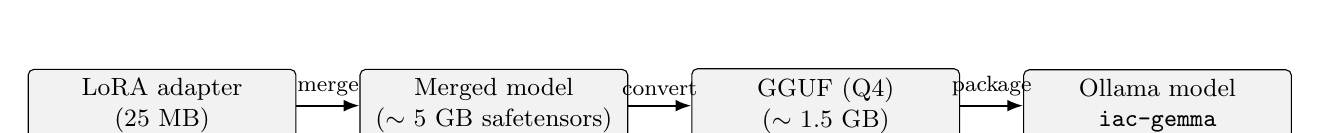
\begin{tikzpicture}[
      node distance=8mm,
      box/.style={draw, rounded corners=2pt, minimum width=3.4cm,
                  minimum height=0.8cm, align=center, font=\small,
                  fill=gray!10},
      arrow/.style={-{Latex[length=2mm]}, thick}
    ]
    \node[box] (adapter)     {LoRA adapter\\(25~MB)};
    \node[box, right=of adapter] (merged)  {Merged model\\($\sim$~5~GB safetensors)};
    \node[box, right=of merged]  (gguf)    {GGUF (Q4)\\($\sim$~1.5~GB)};
    \node[box, right=of gguf]    (ollama)  {Ollama model\\\texttt{iac-gemma}};
    \draw[arrow] (adapter) -- node[above, font=\footnotesize] {merge} (merged);
    \draw[arrow] (merged)  -- node[above, font=\footnotesize] {convert} (gguf);
    \draw[arrow] (gguf)    -- node[above, font=\footnotesize] {package} (ollama);
  \end{tikzpicture}
  \caption{From adapter to deployable Ollama model.}
  \label{fig:integration-path}
\end{figure}

\textbf{Step 1 --- Merge.} A short script using
\texttt{PeftModel.merge\_and\_unload()} fuses the adapter back into the
base weights, producing a self-contained model directory. Storage cost
rises to roughly 5~GB (the size of the full Gemma-2-2B) but this file
never ships: it is an intermediate artefact.

\textbf{Step 2 --- Convert to \gls{gguf}.} The
\texttt{llama.cpp/convert\_hf\_to\_gguf.py} utility translates the merged
\gls{hf} directory into a single \gls{gguf} file. A subsequent
\texttt{llama-quantize} pass reduces it to 4-bit precision (Q4\_K\_M)
and brings the file size down to roughly 1.5~GB. This is what gets
distributed and loaded by Ollama.

\textbf{Step 3 --- Package for Ollama.} A minimal \texttt{Modelfile}
declaring the base \gls{gguf}, the Gemma-2 chat template, and a
security-focused system prompt is passed to \texttt{ollama create
iac-gemma}. Thereafter the model can be invoked identically to any
other Ollama model.

On paper, the only change required on the framework side is to set
\texttt{OLLAMA\_MODEL=iac-gemma} in the \texttt{.env} file: the existing
\texttt{FixGenerator} class (in \texttt{Code/src/generator/fix\_generator.py})
discovers the backend and model through environment variables.
This integration has not yet been exercised end to end and may require
adjustments to the chat template or stop tokens.

\section{Config B Evaluation}

Once the model is live in Ollama, the framework's evaluation script
\texttt{Code/scripts/evaluate.py} can be re-run on the eight-file
labelled dataset to produce \emph{Config B} numbers:

\begin{itemize}
  \item \textbf{Config A} (reported in Rapport~2, Chapter~6):
        Checkov alone. F1~=~0.132, Precision~=~0.084, Recall~=~0.304.
  \item \textbf{Config B} (this report, pending):
        contextual analyzer $+$ fine-tuned \gls{llm} $+$ external
        validator (Checkov), full agentic pipeline.
  \item \textbf{Config C} (deferred):
        same as Config~B with self-consistency (N=5 samples) and
        iterative retrieval refinement.
\end{itemize}

The primary metrics of interest for Config~B, consistent with Rapport~2,
are Patch Validity Rate, Smell Elimination Rate, No-New-Issues Rate,
and a macro-averaged F1 over the ground-truth smell set.

\section{Dataset Quality Improvements}

Regardless of the evaluation outcome, the label-noise analysis of
Chapter~\ref{ch:discussion} motivates an incremental improvement of the
dataset preparation pipeline:

\begin{enumerate}
  \item Add a \texttt{--diff-matches-smell} filter in
        \texttt{01\_prepare\_dataset.py} that keeps only records whose
        diff contains a regex match for the declared smell.
  \item Introduce a separate high-purity corpus consisting only of the
        Checkov and KICS test fixtures (1{,}850 records). Evaluate
        training on this small clean corpus against the larger noisy
        one.
  \item Extend version~2 of the scraper (currently incomplete, introduces
        the GHArchive discovery path) to include a diff-hunk-level
        classifier rather than only a file-level one.
\end{enumerate}

\section{Model Scaling}

If the Config~B measurement, once available, proves insufficient, two
axes of scaling are open:

\begin{itemize}
  \item \textbf{Larger base model}. Qwen2.5-Coder-3B-Instruct is
        listed as a drop-in alternative in our training script; it is
        non-gated and advertised as a code-specialised model.
        Fine-tuning it is, in principle, compatible with Kaggle's T4
        memory budget, but this has not been verified.
  \item \textbf{Longer training}. Two-to-three epochs on the same
        corpus, with early stopping on validation loss. Additional
        GPU-time cost is roughly proportional to the number of epochs.
\end{itemize}

\section{Long-Term Outlook}

The fine-tuning effort described in this report is one building block
in a larger research programme. In the full vision the framework
iterates between \gls{rag}-augmented generation, scanner-based
validation, and selective retraining on the examples the validator
marks as failing. The current experiment validates that the generator
module can be specialised cheaply and deployed locally; it does not by
itself close the loop. Subsequent reports will address self-training
from validator feedback and the introduction of hunk-level label
distillation.

% ============================================================
\chapter{Conclusion}
% ============================================================

This report documents a first, preliminary fine-tuning experiment
carried out within the agentic \gls{iac} security framework proposed in
Rapport~2. From a 31{,}748-record scanner-validated scrape we extracted
a 4{,}050-record subset; we then ran one pass of \gls{qlora} fine-tuning
on \texttt{google/gemma-2-2b-it} --- a small 2~B-parameter base model
--- on Kaggle's free T4~x2 tier (a single device was used by the
training script), observing a training loss of 0.528 and an
evaluation loss of 0.467 in 1~h~47~min. A 25~MB adapter was produced
and manually inspected on three test samples.

The main value of this iteration is methodological: the end-to-end
pipeline (scrape~$\to$~filter~$\to$~train~$\to$~adapter) runs within
the constraints of a free GPU tier, and the dominant obstacle to better
results has been identified as label noise in the commit-scraped
ground truth rather than a property of the model or the training
procedure. No claim of competitive performance is made at this stage.

The immediate next steps are concrete but unexecuted: merge the adapter,
convert it to \gls{gguf}, serve it through Ollama, and run the
framework's evaluation script to produce the first \emph{measured}
Config~B numbers. In parallel, a stricter hunk-level label filter and
an experiment on a scanner-fixture-only subset are planned to test the
label-noise hypothesis directly. Only after these steps will it be
possible to populate Chapter~6 of the final thesis report with a
meaningful Config~A/B/C comparison.

\end{document}
